\documentclass[10pt,conference,compsocconf]{IEEEtran}

\usepackage{hyperref}
\usepackage{amsmath}
\usepackage{graphicx}	% For figure environment
\usepackage{array}
\newcolumntype{p}[1]{>{\centering\arraybackslash}m{#1}}
\usepackage{multirow}
\setlength{\textfloatsep}{8pt}
\setlength{\floatsep}{8pt}
\setlength{\intextsep}{5pt}

\begin{document}

\title{CS433 - Machine Learning Project 1}

\author{
  Francisco Badia Laguillo, Lluc Santamaria Riba, Aleksandra Zawadzka\\
}

\maketitle

\section{Introduction}
Coronary heart disease (MICHD), the narrowing of arteries supplying the heart, is the leading cause of death worldwide \cite{bhf2025}. To study its risk factors, the U.S. Centers for Disease Control established the Behavioral Risk Factor Surveillance System (BRFSS), which collects data on health-related behaviors, chronic conditions (including coronary heart disease), and use of preventive services.

This project aims to develop a machine learning model that predicts an individual’s risk of coronary heart disease using BRFSS data \cite{cdc_brfss2024}, enabling risk assessment based on personal behaviors and health status.

\section{Exploratory Data Analysis}
Initial exploratory data analysis revealed the characteristics and challenges of the dataset. The collection comprises 328,135 samples across 321 features, where the labels encode the MICHD diagnosis (y=1) or no diagnosis (y=-1). A significant challenge is the prevalence of missing data, with 45\% of all entries being NaN values, including 182 features exhibiting a NaN ratio above 10\%. Feature analysis showed 95 were categorical (with $\leq10$ unique values) and 44 were continuous. Furthermore, the dataset presents severe imbalance, with the MICHD diagnosis (y=1) only representing 10\% of all samples. Finally, 64 features were identified as calculated variables (prefixed with an underscore in the feature label).

\section{Feature Processing}
Feature processing was necessary to clean and prepare the data for modeling. To ensure feature reliability, we applied an initial filter, dropping 182 features where the percentage of NaN values exceeded 10\%, leaving 139 features. Features exhibiting zero variance (homogenic) were subsequently removed as they provide no predictive signal. Initially, we used Pearson correlation calculated on the entire dataset to select the most promising features for baseline training. However, this introduced data leakage, as the correlation mask was informed by the yet-to-be-separated testing data, leading to optimistic results on model validation. We corrected this by discarding all predictive feature selection, relying instead on a complete feature set defined purely by data reliability (NaN ratio). All remaining features are processed as follows: calculated variables were retained due to their potential to capture meaningful interactions. 71 main features were processed manually to map values and classify them as categorical or continuous, while the remainder were processed algorithmically. All categorical variables were prepared using one-hot encoding, treating NaNs as a separate category to potentially capture information from the missingness pattern. Finally, the entire training data was split to establish a validation set for model evaluation.

\subsection{Feature standardization}
Initially, z-score standardization was incorrectly applied by calculating the mean ($\mu$) and standard deviation ($\sigma$) over the entire, not-yet-splitted training dataset. This methodology resulted in data leakage, as the training data used parameters that contained knowledge of the distribution of the validation and test sets. We ensured a strict separation of data knowledge calculating $\mu$ and $\sigma$ exclusively from the training partition and then applied to its corresponding validation and test set.


\section{Models and Methods}
This section details the experimental design and the different model families utilized. To ensure robust performance estimates and mitigate against reliance on a single data split, all models are rigorously evaluated using 5-fold Cross-Validation. Unless otherwise specified, training runs were constrained to a maximum of 200 iterations.

\subsection{Linear Regression}
The first model we tried to fit is a linear regression implemented using gradient descent. The simplest version we tried to fit is the regular one.  For this initial setting, the model prediction for all labels is negative. This is because of the imbalance in the labels' distribution in the dataset. We first tried to solve this problem using loss balancing, as shown by this formula:
$$L_{\text{b}} = \frac{1}{N} \left( \frac{N_{\text{neg}}}{N_{\text{pos}}} \sum_{n: y_n=+1} (y_n - \mathbf{x}_n^T\mathbf{w})^2 + \sum_{n: y_n=-1} (y_n - \mathbf{x}_n^T\mathbf{w})^2 \right)$$

Loss balancing to address the data unbalance led to an F1-score of 0.35 and an accuracy of 0.737, the full results are shown in table \ref{tab:results}. This significant improvement proves that data imbalance is one of the main issues to solve. Logistic regression is therefore explored as it better handles class imbalance.

Furthermore, feature expansion yielded no predictive gain over the linear form. This finding suggests the model's capacity, even with basic Linear Regression, is sufficient to capture the underlying patterns, and the relationship between the features and the target is primarily linear. Figure \ref{fig:degrees} illustrates this phenomenon. The performance metrics, F1-Score and Accuracy, remain essentially flat for low polynomial degrees, confirming that added non-linearity offers no benefit. Performance begins to decrease significantly only when the degree is augmented too much (from degree 5 onward). Although the loss curves show a valley (indicating an optimal point), the absolute decrease in loss is negligible, reinforcing that the model gains minimal explanatory power from the expanded terms.

\begin{figure}[htbp]
    \centering
    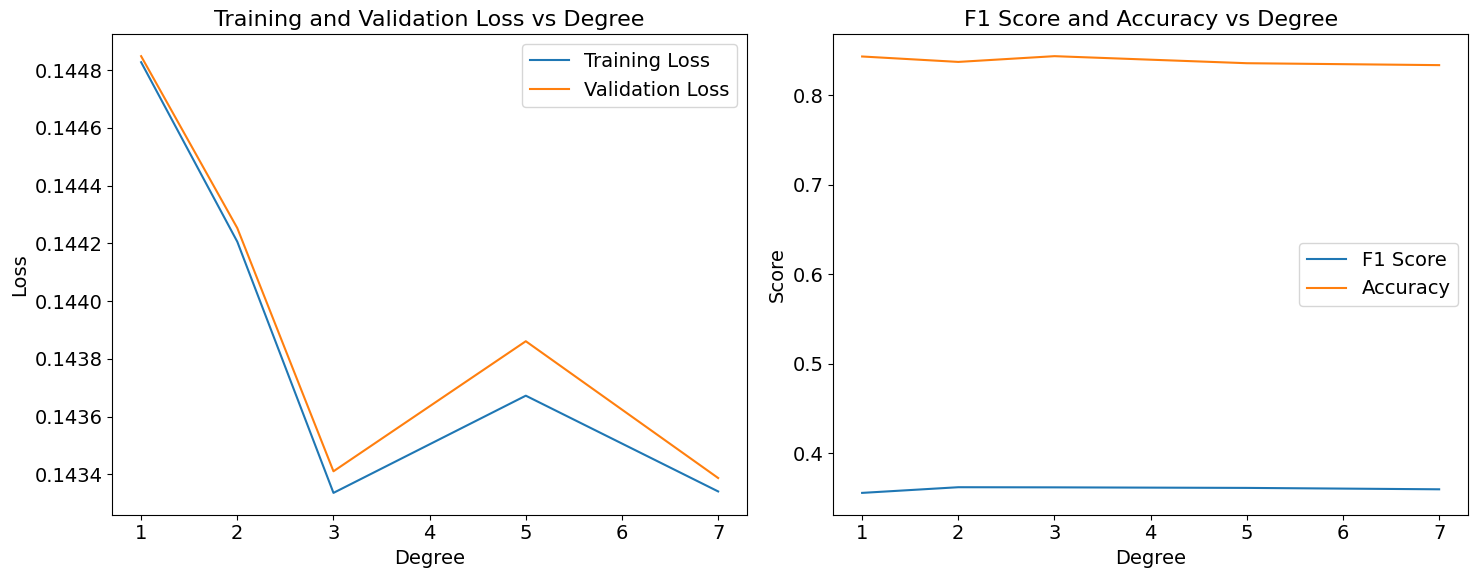
\includegraphics[width=0.5\textwidth]{degrees.png}
    \caption{Training and validation losses, F1-score and accuracy versus degree of feature expansion for linear regression model.}
    \label{fig:degrees}
\end{figure}


\subsection{Logistic Regression}
Logistic Regression (LogR) was selected as a powerful and appropriate model because its inherent probabilistic nature handles binary classification and data imbalance very effectively. Initially the decision threshold for making the predictions was fixed at $0.5$, performance was initially poor. We decided to adjust the prediction threshold using cross-validation, aiming to maximize the F1-score through a grid search. Results improved substantially after implementing a fold-specific threshold optimization: for each cross-validation fold, the optimal decision threshold was determined by selecting the value that maximized the F1-score.

We then explored the impact of the learning rate ($\gamma$) on performance, identifying and using the best threshold separately for each value of, $\gamma$ as explained above (Figure \ref{fig:gamma_LogR}). With a maximum training limit of 300 iterations for each run, the model proved highly robust, maintaining good F1-scores across a wide range of $\gamma$ values. Performance deteriorates only at the extremes: for very low $\gamma$ (due to insufficient convergence within the iteration limit) and for very high $\gamma$ (where the optimization process begins to diverge).

\begin{figure}[htbp]
    \centering
    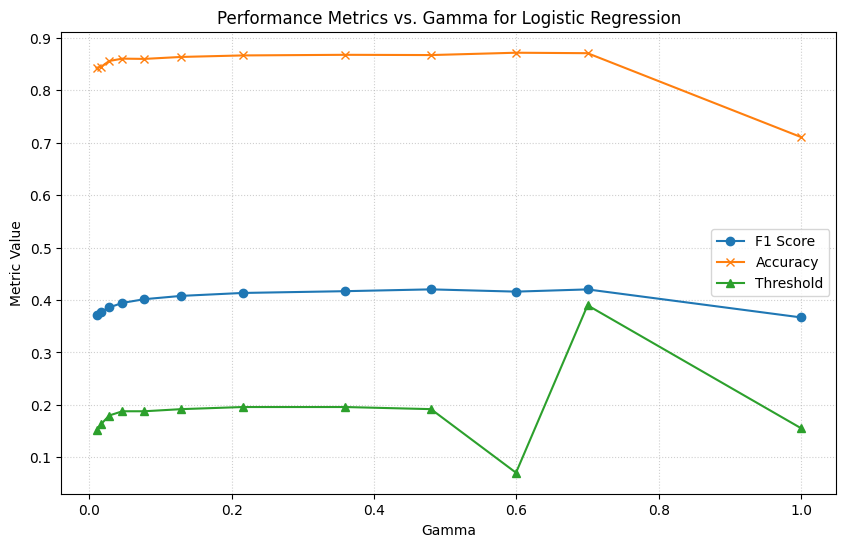
\includegraphics[width=0.45\textwidth]{gamma_LogR.png}
    \caption{Accuracy and F1-score at different values of Learning Rate ($\gamma$) for Logistic Regression (300 Iterations). Decision thresholds maximising the F1-score at the given $\gamma$ are also shown.}
    \label{fig:gamma_LogR}
\end{figure}


\subsection{Mitigating data imbalance}
The improvements observed with threshold adjustment in logistic regression led us to investigate whether this method could also improve results in linear regression model, which has been subsequently tested. Loss balancing is also tested in logistic regression by multiplying the loss term by $\frac{N_{\text{neg}}}{N_{\text{pos}}}$ for positive labels. Table \ref{tab:results} shows the results for both linear and logistic regression:

\begin{table}[h]
\centering
\begin{tabular}{|p{1.2cm}|p{1cm}|p{1cm}|p{1cm}|p{1cm}|p{0.8cm}|}

\hline
 & \textbf{Metric} & \textbf{No Treatment} & \textbf{Loss Balancing} & \textbf{Threshold Adjustment} & \textbf{Both} \\ \hline
\multirow{2}{1.4cm}{\textbf{Linear Regression}} &  F1-score & 0 & 0.347 & 0.402 & 0.410 \\ \cline{2-6}
  & Accuracy & 0.910 & 0.737 & 0.858 & 0.880 \\ \hline
\multirow{2}{1.4cm}{\textbf{Logistic regression}} &  F1-score & 0.420 & 0.395 & 0.424 \footnotemark & 0.412 \\ \cline{2-6}
 &  Accuracy & 0.892 & 0.894 & 0.868 & 0.859 \\ \hline


\end{tabular}
\caption{Metrics obtained for different balancing treatments for linear and logistic regressions}
\label{tab:results}
\end{table}

\footnotetext{This best results, reported in the table and reproduced on our best submission on AIcrowd, were achieved using extended runs of functions that optimize hyperparameters. The current run.py execution yield slightly lower results, as they are designed to reduce runtime. For instance, the best submission used Logistic Regression with $search\_threshold\_iterations=1000$, $\gamma = 0.7$ and $max\_iters=750$.}

Linear and logistic regression show similar best metrics, though logistic regression is more robust, likely due to its inherent resistance to class imbalance. Loss balancing offers no benefit, while threshold adjustment improves both models, reflecting its model-agnostic nature.
\vspace{-0.5em}

\section{Conclusion}
The top-performing model, logistic regression with threshold adjustment, achieved an accuracy of 0.868 and an F1-score of 0.424. Model performance was strongly affected by data imbalance, requiring countermeasures for data imbalance, from which threshold adjustment proved to be the most effective. Feature expansion did not improve results, indicating that the relationships in the data are largely linear. As expected, logistic regression excelled overall, being well-suited for binary classification and robust to imbalanced data.

Focusing on real-life patient diagnosis, we must prioritize minimizing False Negatives (missed diagnoses), as this represents the greatest patient risk. As a future extension, reducing the current 45\% recall failure (missing 45\% of MICHD cases) should be a key priority for model refinement.


\bibliographystyle{IEEEtran}
\bibliography{literature}

\end{document}
